
%(BEGIN_QUESTION)
% Copyright 2011, Tony R. Kuphaldt, released under the Creative Commons Attribution License (v 1.0)
% This means you may do almost anything with this work of mine, so long as you give me proper credit

Calculate the following test-point voltages (all with respect to ground), given a PV signal of 2.8 volts, a SP signal of 2.5 volts, a gain of 1 (pot $R_2$ in mid-position), a bias signal of -3.0 volts (measured at TP6), and all switches placed in the positions as shown in the diagram:

$$\includegraphics[width=15.5cm]{i00897x01.eps}$$

\begin{itemize}
\item{} $V_{TP3}$ = \underbar{\hskip 50pt} volts
\vskip 10pt
\item{} Output = \underbar{\hskip 50pt} volts
\vskip 10pt
\item{} $V_{TP10}$ = \underbar{\hskip 50pt} volts
\vskip 10pt
\item{} $V_{TP5}$ = \underbar{\hskip 50pt} volts
\end{itemize}

\underbar{file i00897}
%(END_QUESTION)





%(BEGIN_ANSWER)

Each correct answer is worth 2.5 points:

\begin{itemize}
\item{} $V_{TP3}$ = {\bf 2.8} volts 
\vskip 10pt
\item{} Output = {\bf 2.7} volts 
\vskip 10pt
\item{} $V_{TP10}$ = {\bf 0} volts
\vskip 10pt
\item{} $V_{TP5}$ = {\bf -0.3} volts
\end{itemize}

%(END_ANSWER)





%(BEGIN_NOTES)

{\bf This question is intended for exams only and not worksheets!}.

%(END_NOTES)


